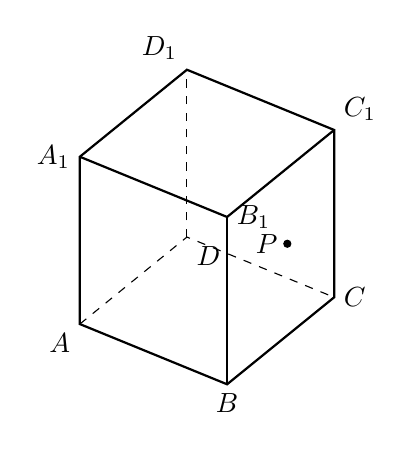
\begin{tikzpicture}[>=stealth, scale=0.85]
  % 顶点坐标
  \coordinate (A) at (0, 0);
  \coordinate (B) at (2.2, -0.9);
  \coordinate (C) at (3.8, 0.4);
  \coordinate (D) at (1.6, 1.3);
  \coordinate (A1) at (0, 2.5);
  \coordinate (B1) at (2.2, 1.6);
  \coordinate (C1) at (3.8, 2.9);
  \coordinate (D1) at (1.6, 3.8);

  % 侧面 BB1C1C 内动点 P
  \coordinate (P) at (3.1, 1.2);

  % 虚线（不可见棱）
  \draw[dashed, thin] (A) -- (D) -- (C);
  \draw[dashed, thin] (D) -- (D1);

  % 实线（可见棱）
  \draw[thick] (A) -- (B) -- (C) -- (C1) -- (D1) -- (A1) -- cycle;
  \draw[thick] (B) -- (B1);
  \draw[thick] (A1) -- (B1) -- (C1);

  % 动点 P 及其标注
  \filldraw[black] (P) circle (1.5pt);
  \node[left] at (P) {$P$};

  % 顶点标签
  \node[below left] at (A) {$A$};
  \node[below] at (B) {$B$};
  \node[right] at (C) {$C$};
  \node[below right] at (D) {$D$};
  \node[left] at (A1) {$A_1$};
  \node[right] at (B1) {$B_1$};
  \node[above right] at (C1) {$C_1$};
  \node[above left] at (D1) {$D_1$};
\end{tikzpicture}
